\section{Desired model}

The desired model will provide a setting for which we can explore fundamental resource and performance properties of the \xcloud{} in a system of mobile \ues{}. The mobile \ues{}, radio access network, and service application will subject the \dcs{} with a load characteristic for generic mobile phone traffic and the type of services that might be deployed to the \xcloud{}.

\begin{figure}[tb]
	\centering
	\includegraphics[width=\linewidth]{desiard_model.eps} 
	\caption{Performance model}
	\label{fig:performance_model}
\end{figure}

As the topology of any future \xcloud{} or proposed forthcoming mobile networks is yet to be determined, in this paper we propose a generic telecom infrastructure model that disregards generational specific properties such as those found in the physical layer and cell load-balancing methods. Nevertheless, conceivably and in order to confine the geographic domain of the model adheres to current general LTE cell planing practices. 

In order to explore the fundamental dynamics of mobility in the generic case, the model does not adhere to any soci-demographic patterns or urban topologies. To the same effect, the mobile network base stations are uniformly distributed across its 2-dimensional domain.

Similarly, in order to represent the variety of possible services, the service model needs to generate traffic that is characteristic for a generic \ue{}. Additionally, the generated traffic shall therefore be provided by a stochastic process that is also independent of location.

The concert of the mobility model and the service model in a uniformly distributed mobile network that will provide the modeled \dcs{} with relevant request load. It is worth reiterating that the traffic load is more relevant to our investigation than specific topological and network properties.

The \dc{} model will host multiple VMs that will process the arriving requests corresponding to its service commitment. Additionally, when a VM is migrated between \dcs{} it shall incur a load on the both \dcs{}. Furthermore, the resources within a \dc{} are shared amongst the receding VMs, the amount of compute resources dedicated to one service is thus proportional to the number of services hosted in that \dc{}.  Minute memory management, interference, and cross-talk are not fundamental performance properties at this scale and are therefore not modeled.